%
% The first command in your LaTeX source must be the \documentclass command.
\documentclass[sigconf]{acmart}
% \usepackage{amsmath,amsfonts,stmaryrd} % Math packages
% \usepackage{subfigure}
\usepackage{gensymb}
\usepackage{pgfgantt}
% \usepackage{algpseudocode}
% \usepackage{amssymb}
% \usepackage{array}
% \usepackage{bm} % for the bold font Greek symbols in math mode
% \usepackage{breakurl}
% \usepackage{color}
% \usepackage{comment}
% \usepackage{epsfig}
% \usepackage{graphicx}
% \usepackage{hyperref}
% \usepackage{mdwmath} % part of Mark Wooding's powerful
% \usepackage{mdwtab}  % tools for math, tables, ...
% \usepackage{multirow}
% \usepackage{psfrag}
% %\usepackage{times}
% \usepackage{verbatim}
% \usepackage{xspace}
% \usepackage{url}
% \usepackage{enumerate} % Custom item numbers for enumerations


\usepackage{listings} % File listings, with syntax highlighting
\lstset{
	basicstyle=\ttfamily, % Typeset listings in monospace font
}
%
% defining the \BibTeX command - from Oren Patashnik's original BibTeX documentation.
\def\BibTeX{{\rm B\kern-.05em{\sc i\kern-.025em b}\kern-.08emT\kern-.1667em\lower.7ex\hbox{E}\kern-.125emX}}
    
% Rights management information. 
% This information is sent to you when you complete the rights form.
% These commands have SAMPLE values in them; it is your responsibility as an author to replace
% the commands and values with those provided to you when you complete the rights form.
%
% These commands are for a PROCEEDINGS abstract or paper.
% \copyrightyear{2018}
% \acmYear{2018}
% \setcopyright{acmlicensed}
% \acmConference[Woodstock '18]{Woodstock '18: ACM Symposium on Neural Gaze Detection}{June 03--05, 2018}{Woodstock, NY}
% \acmBooktitle{Woodstock '18: ACM Symposium on Neural Gaze Detection, June 03--05, 2018, Woodstock, NY}
% \acmPrice{15.00}
% \acmDOI{10.1145/1122445.1122456}
% \acmISBN{978-1-4503-9999-9/18/06}

%
% These commands are for a JOURNAL article.
%\setcopyright{acmcopyright}
%\acmJournal{TOG}
%\acmYear{2018}\acmVolume{37}\acmNumber{4}\acmArticle{111}\acmMonth{8}
%\acmDOI{10.1145/1122445.1122456}

%
% Submission ID. 
% Use this when submitting an article to a sponsored event. You'll receive a unique submission ID from the organizers
% of the event, and this ID should be used as the parameter to this command.
%\acmSubmissionID{123-A56-BU3}

%
% The majority of ACM publications use numbered citations and references. If you are preparing content for an event
% sponsored by ACM SIGGRAPH, you must use the "author year" style of citations and references. Uncommenting
% the next command will enable that style.
%\citestyle{acmauthoryear}
\renewcommand{\baselinestretch}{1.05}
%
% end of the preamble, start of the body of the document source.
\begin{document}

%
% The "title" command has an optional parameter, allowing the author to define a "short title" to be used in page headers.
\title{Research Proposal: 6-DoF Immersive Video Streaming to Head-Mounted Displays}

%
% The "author" command and its associated commands are used to define the authors and their affiliations.
% Of note is the shared affiliation of the first two authors, and the "authornote" and "authornotemark" commands
% used to denote shared contribution to the research.
\author{Tse-Hou Hung}
\email{tsehou.nthu@gmail.com}
\affiliation{%
  \institution{National Tsing Hua University}
  \city{Hsinchu}
  \state{Taiwan}
}

\begin{abstract}
  Six Degree-of-Freedom (6DoF) Immersive video streaming is very challenging due to various data representations, 
  strict network condition and computing requirements ,and complex user experience models. In my PhD 
  study, we study on three research problems to overcome these three challenges.
  First, we study different data representations to understand their pros, cons, and suitable 
  usage scenarios. Second, we optimize the streaming systems to reduce the bandwidth requirements in immersive video streaming.
  Last, we design and conduct a series of user studies to derive the user experience.
  The results of these three steps lead to a fully-optimized immersive video streaming systems,
  which are crucial to many novel applications, including holographic conferences, 
  real scene streaming, remote surgery, and fire fighter (or military) training.
\end{abstract}
%
% This command processes the author and affiliation and title information and builds
% the first part of the formatted document.
\maketitle
\section{Introduction}\label{sec:intro}
Virtual Reality (VR) technology is thriving in various business sectors,
including computer games, tourism industry, real estates, and occupational trainings. 
The VR scenes can either be generated with computer graphics or captured from nature scenes, 
which provide omnidirectional, a.k.a. 360{\degree}, viewing experience of virtual worlds. 
It is estimated that the global VR market size will reach 26.89 billion USD by 2022, 
with an annual growth rate of 54\% from 2017 to 2022~ \cite{VR_market}.
As VR technology becomes more and more mature, 
researchers start to study its Quality of Experience (QoE) in order to deliver higher-quality scenes for better user experience.

\begin{figure}[tbh]
	\begin{center}
		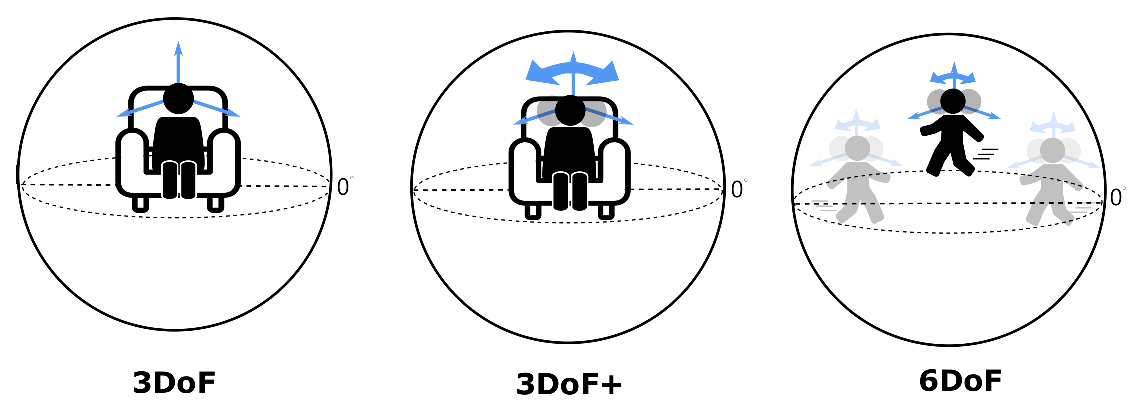
\includegraphics[width=.5\textwidth]{fig/vr_phase}
		\caption{Three phases of VR technology development. The spheres represent the virtual worlds.}
		\label{fig:vr_phase}
	\end{center}
\end{figure}

% Difference between 3DoF+ and 6DoF
One key factor affecting the QoE of VR technology is the way users interact with the virtual worlds. 
MPEG-I group has defined three development phases of the VR technology: 3 Degree-of-Freedom (3DoF), 3DoF+, and 6DoF, which are illustrated 
in Fig.~\ref{fig:vr_phase}.
3DoF VR technology allows users to rotate their heads in three dimensions, which are represented by yaw $\psi$, pitch $\theta$, and roll $\phi$. 
However, with 3DoF VR, when users move their heads or stand up and walk, their position changes do {\em not} affect the views rendered in the 
Head-Mounted Displays (HMDs).
To overcome this limitation, 3DoF+ VR is proposed to support {\em limited} movements.
Namely, users can slightly move their heads to a certain extent when sitting on fixed chairs. 
6DoF VR further enables users to freely move, e.g., walk, in virtual worlds.
Users can not only rotate their heads in three dimensions but also move in the three additional dimensions, which are $x$, $y$, $z$ coordinates. 

A naive way to achieve 3DoF+ and 6DoF is to capture multiple 360$^{\circ}$ videos at different positions~\cite{CSSF18,PZWL+19}, 
and only allow the HMD users to 
switch among these discrete positions in the scenes.
We target more general 3DoF+ and 6DoF VR, where users can freely move in among the discrete positions.
We refer to the streaming systems that support such 3DoF+ and 6DoF VR as {\em immersive video streaming} throughout this proposal.

Achieving real immersive video streaming is not an easy task, because there are many challenges that need to be overcome:
\begin{itemize}
	\item {Different Data Representations: } Various data types can be used to store the information of immersive video, e.g.,
	2D texture and depth image, light field, 3D point cloud, and 3D mesh. Each of them has pros, cons, and usage scenarios, which have not been comprehensively studied.
	\item {Strict Network Condition Requirements: } The data representations of immersive video have a huge data size. 
	They need a lot of bandwidth to be streamed, while the realtimeness needs to be maintained. 
	Take light field video as an example, streaming it consumes bandwidth in the range between 
	200 Gb/s and 1 Tb/s \cite{CVRW+20}, which is much higher than the available bandwidth we have today.
	Moreover, the interactive applications, e.g., 6DoF VR games and holographic conferences, need low latency to realize real-time communications.
	This in turn makes the network condition requirements more strict.
	\item {Complex User Experience Models: } User experience is the quality perceived by  users. 
	It is an important performance metric for multimedia applications.
	However, the user experience of immersive videos is still not explored,
	and the challenges of measuring user experience include but not limited to: 
	(i) too many parameters may affect the user experience in immersive video streaming
	and (ii) it's hard to build an immersive video streaming testbed.
	% Estimating the user experience can help us find the pattern of user habit. 
	% We can reduce the video quality of user not sensitive part to save the network and computing resources.
	
\end{itemize}
% To achieve real immersive video streaming, there are some candidate of data representations:
% XXX todo intro. these data type XXX 
% \begin{itemize}
% 	\item {\bf Depth Image Based Rendering (DIBR): }
% 	\item {\bf Light Field: }
% 	\item {\bf 3D Point Cloud: }
% 	\item {\bf 3D Mesh: }
% \end{itemize}

In this research proposal, we propose three research directions to address the three challenges:
(i) {\em Data Representations} 
(ii) {\em Optimal Streaming} 
(iii) {\em Quality of Experience}. 
We introduce them in details below.
% In our first work \cite{mm20_tr},
% we use Test Model for Immersive Video (TMIV)~\cite{mpeg_N18470,mpeg_N18577,mpeg_N18795}, 
% which is a DIBR codec for immersive video streaming from MPEG, to optimize the immersive video streaming.
% we develop algorithms to solve the configuration optimization problem based on deep learning, particularly the Neural Network (NN) approaches.
% The two proposed algorithms are:
% a Convolutional Neural Network (CNN) based algorithm and a Deep Reinforcement Learning (DRL) based algorithm
% \footnote{We refer to them as CNN and DRL algorithms for short in the rest of this paper.}.
% Our CNN algorithm benefits from: (i) automatic extracting latent features and 
% (ii) inferencing the prediction rapidly and directly according to the input, which allows the configuration optimizer to 
% adapt to various video scenes and dynamic camera parameters.
% Our DRL algorithm systematically builds an {\em agent} that can adapt to dynamic {\em environments}~\cite{SB18,PZWL+19,HZZS18,CIZI+19}.
% The trained agent learns how to quickly search through a large space for optimal configurations. 
% The two proposed algorithms are
% trained to adaptively find the optimal configurations given the diverse video content, HMD user behaviors, and user-specified utility functions.

% Our paper makes the following contributions:
% \begin{itemize}
% \item We propose the first NN-based algorithms\footnote{We also refer to NN-based algorithms as NN algorithms for brevity.} designed for configuration
% optimization of TMIV. Our solution approach can be readily adapted to other
% usage scenarios and immersive video systems.
% \item We conduct extensive experiments with real datasets to evaluate the
% performance of our algorithms. Our objective experiments show that the proposed
% algorithms consume less resources compared to the default and optimal TMIV
% configurations.
% \item We conduct a user study to subjectively evaluate the synthesized view
% quality among configurations generated by different algorithms.
% A detailed analysis shows
% that the difference of the synthesized view quality is insignificant among them.
% \end{itemize}
% We submitted our paper to ACM Multimedia Conference 2020.

\section{Research Problems}
\subsection{Data Representations}\label{sec:data_representation}

Whiles data types mentioned in Sec.~\ref{sec:intro} could be suitable to immersive video streaming,
Their pros and cons are unknown.
In our research group, we have studied 3DoF VR streaming in the past few years \cite{FYHH20,FLPH19}. 
These works help us to understand the existing streaming techniques in 3DoF 360{\degree} video streaming.
We are currently expand our research to different 6DoF data types to understand their pros and cons.
We will also concretize their suitable usage scenarios,
The final outcome of this work is several immersive video streaming testbeds that support heterogeneous data representations.
Through real experiments, we hope to know more systems challenges in these emerging applications.
\subsection{Optimal Streaming}\label{sec:optimal_streaming}

To reduce the bandwidth requirement of immersive video streaming, the streaming systems must be optimized.
In our recent work \cite{mm20_tr},
we use Test Model for Immersive Video (TMIV)~\cite{mpeg_N18470,mpeg_N18577,mpeg_N18795}, 
which is a Depth Image Based Rendering (DIBR) codec for immersive video streaming from MPEG, to optimize the immersive video streaming.
We develop algorithms to solve the configuration optimization problem based on deep learning, particularly the Neural Network (NN) approaches.
The two proposed algorithms are:
a Convolutional Neural Network (CNN) based algorithm and a Deep Reinforcement Learning (DRL) based algorithm
\footnote{We refer to them as CNN and DRL algorithms for short in the rest of this paper.}.
Our CNN algorithm benefits from: (i) automatic extracting latent features and 
(ii) inferencing the prediction rapidly and directly according to the input, which allows the configuration optimizer to 
adapt to various video scenes and dynamic camera parameters.
Our DRL algorithm systematically builds an {\em agent} that can adapt to dynamic {\em environments}~\cite{SB18,PZWL+19,HZZS18,CIZI+19}.
The trained agent learns how to quickly search through a large space for optimal configurations. 
The two proposed algorithms are
trained to adaptively find the optimal configurations given the diverse video content, HMD user behaviors, and user-specified utility functions.
We submitted our paper to ACM Multimedia Conference 2020, which is under review.

We are currently extending this work into a journal submission. 
In particularly, we plan to (i) design, implement, and evaluate an end-to-end DIBR-based immersive video streaming system,
(ii) apply the state-of-the-art DRL algorithms and (iii) adopt larger datasets to train our optimizers.
We expect the performance of our systems can be better after we apply these optimizations.
Moreover, according to the research outcomes of Sec.~\ref{sec:data_representation}, 
% we also study the new streaming technique to address the challenges in these data types.
we will generalize our solutions to other data types.
\subsection{Quality of Experience (QoE)}
To measure QoE of users, we plan to design and conduct a series of user studies  
to quantify the relationship between each parameters and user experience in immersive video streaming sessions.
In our previous work \cite{mm20_tr}, we conduct a small-scale user study to evaluate our solution.
The testbed used in that work can be extended and used in more comprehensive subjective experiments.
The high-level architecture of the immersive video streaming system is shown in Fig.~\ref{fig:architecture}.
Moreover, we plan to measure the Just-Noticeable Difference (JND)~\cite{JLK06} bitrate of immersive video streaming.
Using JND bitrates, we can intelligently save the network and computing resources without affecting the user experience.
Combining the outcomes of the QoE study with the ones achieved in Sec.~\ref{sec:data_representation} and Sec.~\ref{sec:optimal_streaming}
gives a fully-optimized immersive 6DoF video streaming system.
\begin{figure}[tbh]
	\begin{center}
		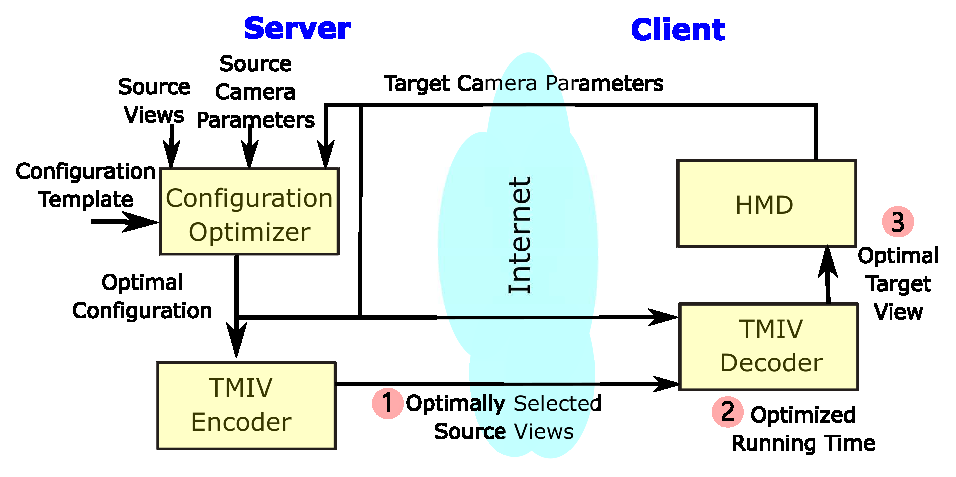
\includegraphics[width=.5\textwidth]{fig/architecture}
		\caption{High-level architecture of immersive video streaming systems for our QoE study.}
		\label{fig:architecture}
	\end{center}
\end{figure}
% If we figure out which level of distortion can tolerate by user, we can choose suitable quality to stream.
% In this way, the bandwidth consumption can be reduced, and the user can perceive the great quality in the same time.
% % However, measuring QoE in immersive video is harder than traditional 2D video or 360{\degree} video.
% The immersive video is the new interactive way in VR,
% so measuring QoE in immersive video is not be researched comprehensively.
% However, it is harder than traditional 2D video or 360{\degree} video.
% In 2D video, the user see the same content on the screen.
% In immersive video and 360{\degree}, user can watch video in different positions and/or orientations by HMD. 
% Each user may see the different content in the video. It makes analyzing the general QoE pattern hard.

% In this research plan, we plan to design a series of experiments to analyze the QoE and user pattern in immersive video.
% We will try different method to overcome the aforementioned problem, 
% including record the trajectory of viewport of subjects, guide subjects where should watch etc..
% Moreover, we plan to measure the Just-Noticeable Difference (JND)~\cite{JLK06} in immersive video.
% In this way, we can find the "sweet point" between QoE and bandwidth consumption.



% \subsection*{First Year: TMIV Immersive Video Streaming System and Explore Data type of 6DoF}
% Given that the current research is the first work trying to optimize the TMIV configurations, we believe
% it will stimulate many more systems research in immersive video streaming. Nevertheless, several crucial
% challenges still need to be overcomed in our first work.
% \begin{itemize}
%     \item {\bf immersive video streaming system:} Currently, because of the high demand for bandwidth
%     and computing resources, build the complete immersive video streaming system is still challenging.
%     In future work, to address the challenges, we add the configuration optimizer into the
%     system. We also design the threshold of bandwidth consumption to limit the maximum of data size.
%     Moreover, we use GPU to process the computation in the system parallelly.
%     \item {\bf State-of-the-art RL algorithm:} In our current work, we choose Deep Q-learning (a.k.a. Deep QNetwork,
%     DQN) to train the DRL configuration optimizer. The experiment shows that DQN achieves
%     better performance. However, there are some methods we haven’t try, e.g., policy gradient, Asynchronous
%     Advantage Actor-critic (A3C). In future work, we seek more powerful DRL algorithms to
%     improve the performance of our DRL optimizer.
%     \item {\bf More experienced optimizer:} In future work, to let our optimizer more general, we train our agent
%     with more datasets. We use more different datasets so that optimizer can choose the best option in
%     most of situation, even the situation they never meet it.
% \end{itemize}

% Moreover, the other data types mention in Sec.~\ref{sec:motivation} also have big potential to be 
% the ideal data representation in immersive video streaming. 
% We plan to study all of 6DoF data types comprehensively to figure out their pros. and cons..
% We also analyze the research problem in each 6DoF data type, respectively.
% % After that, we can know the most important problem in immersive video streaming.

% \subsection*{Second Year: Quality of Experience in Immersive Video Streaming}

% Quality of Experience (QoE) study is important in immersive video streaming. 
% If we figure out which level of distortion can tolerate by user, we can choose suitable quality to stream.
% In this way, the bandwidth consumption can be reduced, and the user can perceive the great quality in the same time.
% % However, measuring QoE in immersive video is harder than traditional 2D video or 360{\degree} video.
% The immersive video is the new interactive way in VR,
% so measuring QoE in immersive video is not be researched comprehensively.
% However, it is harder than traditional 2D video or 360{\degree} video.
% In 2D video, the user see the same content on the screen.
% In immersive video and 360{\degree}, user can watch video in different positions and/or orientations by HMD. 
% Each user may see the different content in the video. It makes analyzing the general QoE pattern hard.

% In this research plan, we plan to design a series of experiments to analyze the QoE and user pattern in immersive video.
% We will try different method to overcome the aforementioned problem, 
% including record the trajectory of viewport of subjects, guide subjects where should watch etc..
% Moreover, we plan to measure the Just-Noticeable Difference (JND)~\cite{JLK06} in immersive video.
% In this way, we can find the "sweet point" between QoE and bandwidth consumption.

% \subsection*{Third Year: Optimize Immersive video streaming}

% Using ABR, synthesis or other method to reduce bandwidth demand and latency.

% \subsection*{Forth Year: Real-Time Immersive Video Streaming System}

% Build the Real-Time Immersive Video Streaming System.




% In second year, we want to propose some new algorithms and techniques to deal with the challenges in 6DoF VR streaming.
% This challenges including but not limited: 
% \begin{itemize}
%     \item {\bf high bandwidth consumption and storage space demand: } The 6DoF data type usually have huge data size, because they have to
%     include all of information in the scene. Take light field video for example, it's expected to require bandwidth in the range between 200 Gb/s 
%     and 1 Tb/s \cite{CVRW+20}, which higher than the highest bandwidth we can achieve today. 
%     \item {\bf low latency demand: } To achieve real-time 6DoF VR video streaming, the low and stable latency is needed. Especially in 
%     interactive application, e.g., holographic conference, gaming. 
% \end{itemize}
% Although there are some existing research work on them \cite{CVRW+20}, it still have lots of problem and challenge need to  be addressed.





\section{Research Plan}
% \begin{figure}[tbh]
% 	\begin{center}
% 		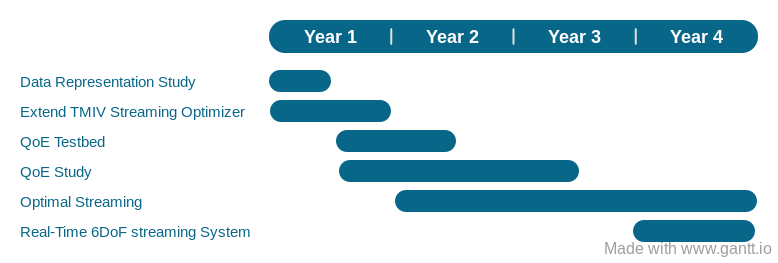
\includegraphics[width=.5\textwidth]{fig/gantta}
% 		\caption{Gantt chart of research plan.}
% 		\label{fig:Gantt}
% 	\end{center}
% \end{figure}
\begin{figure}[tbp]
	\begin{center}
	\begin{ganttchart}[y unit title=0.4cm,
	y unit chart=0.5cm,
	vgrid,hgrid, 
	title label anchor/.style={below=-1.6ex},
	title left shift=.05,
	title right shift=-.05,
	title height=1,
	bar/.style={fill=gray!50},
	incomplete/.style={fill=white},
	progress label text={},
	bar height=0.7,
	group right shift=0,
	group top shift=.6,
	group height=.3,
	group peaks={}{}{.2}]{1}{8}
	\gantttitle{Year 1}{2}
	\gantttitle{Year 2}{2}
	\gantttitle{Year 3}{2}
	\gantttitle{Year 4}{2} \\

	\ganttbar{Data Representations}{1}{1} \\
	\ganttbar{Extend TMIV Streaming Optimizer}{1}{2} \\
	\ganttbar{QoE Testbed}{2}{3} \\
	\ganttbar{User Study}{2}{6} \\
	\ganttbar{Optimal Streaming}{3}{8} \\
	\ganttbar{Real-Time 6-DoF Streaming System}{7}{8} \\
	\end{ganttchart}
	\end{center}
	\caption{Gantt Chart}
	\label{fig:Gantt}
\end{figure}

Fig.~\ref{fig:Gantt} gives the Gantt chart of my research plan.
The first problem is the data representation study.
The outcome of this research problem is our better understanding on the immersive video streaming systems, which is also useful to the research community.
Concurrently, We extend our recent work \cite{mm20_tr} to turn it into a journal paper.
After that, we work on the QoE study. We plan to build an immersive video streaming testbed and
conduct a series of user studies to understand the user experience.
We will also continue optimizing the immersive video streaming testbed by applying different optimization algorithms developed by us.  
The results of QoE study can also help us better optimize the testbed.
Last, we will design, build, and evaluate a real-time immersive video streaming system based on the results of our research 
to turn it into a journal paper.
% XXX add gantt chart at here XXX
\section{Expected Impacts}
% one paragraph on what's current stage before my work
Currently, the techniques of immersive video streaming are still in their infancy.
% Most of the challenges mentioned in front sections haven't solved yet, especially the high bandwidth requirement.
Most of the challenges identified in this proposal have not been rigorously studied.
Existing VR/AR applications do not support real-time streaming; 
Even if they do, only 3DoF interactions are supported, which is not the {\em real} immersive experience.

% one paragraph on what it will become after my work 
In my PhD study, we will propose a series of solutions to overcome the challenges of immersive video streaming.
As system researchers, these solutions through actual experiments. 
In data representation research, we will provide a comprehensive review, 
which can help the research community gain more knowledge on the features, challenges and opportunities of various 6DoF data types.
Through user study and data analysis, we will find new discoveries on the user experience of immersive video streaming in QoE research.
With these discoveries, the content creators can better meet users' needs when they create the immersive content.
The researchers can also use the users' viewing behavior to develop more efficient streaming solutions.
In optimal streaming, we will propose innovative algorithms to overcome various issues caused by scarce resources.
The bandwidth and latency requirements of immersive video streaming will, therefore, fulfilled under diverse network conditions, and
several 6DoF applications can be realized.

\begin{figure}[tbh]
	\begin{center}
		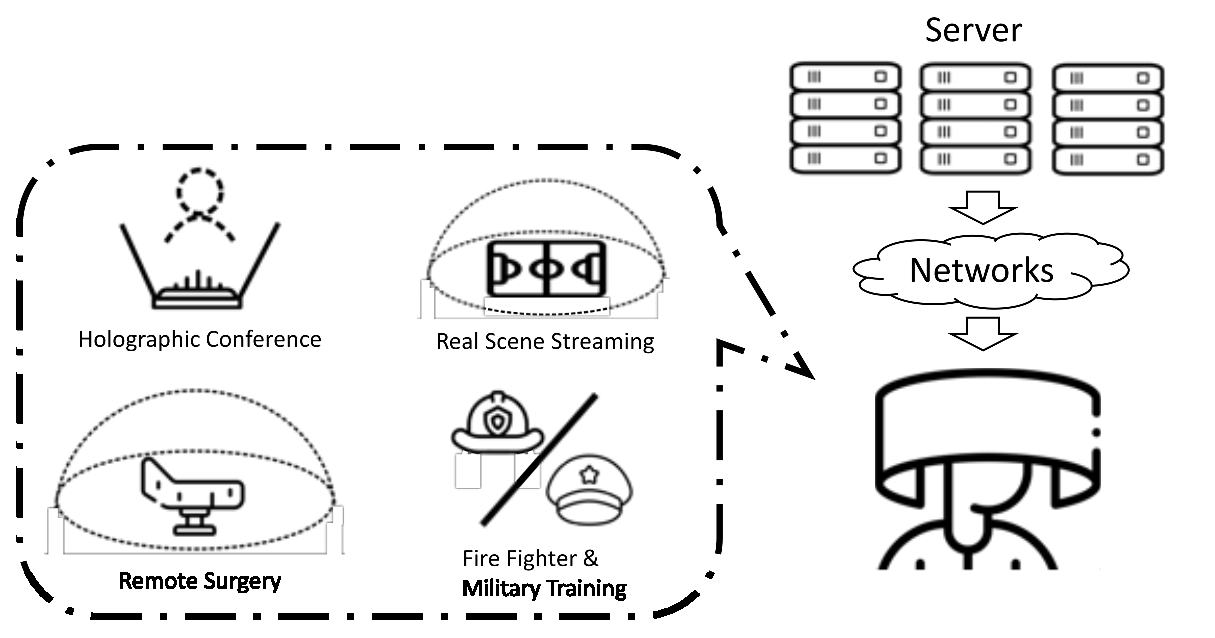
\includegraphics[width=.5\textwidth]{fig/usage_scenario}
		\caption{Usage scenario of immersive video streaming.}
		\label{fig:usage_scenario}
	\end{center}
\end{figure}

% one paragraph on how would my work change people life 
The techniques of immersive video streaming can make people's life more convenient and productive.
As shown in Fig.~\ref{fig:usage_scenario}, immersive video streaming can be used in various usage scenarios.
\begin{itemize}
    \item {\bf Holographic conferences} may become reality. 
    Users can see the projection of remote people and communicate with  one another naturally.
    The holographic conferences will provide exactly the same experience as face-by-face.
    \item {\bf Real scene streaming} may provide immersive live streaming for sports, speech, and other events. 
    For example, users can watch live sports without blind angles to enjoy the games.
    \item {\bf Remote Surgery} can also be performed. 
    Immersive video streaming can provide the situations of remote patients to 
    the doctor, who can carry out the surgery remotely. This will improve the healthcare quality in rural areas.
    \item {\bf Fire fighter and Military training} can be clone in a safer and more efficient way. 
    The training sessions can simulate real situations to help learners experience danger environments without risks.
\end{itemize}


% The usage scenario of immersive video streaming shown in Fig.~\ref{fig:usage_scenario}.


% The next two lines define the bibliography style to be used, and the bibliography file.
\bibliographystyle{ACM-Reference-Format}
\bibliography{refs}

\end{document}
